% !TeX TS-program = lualatex -interaction=nonstopmode % | txs:///view-pdf | txs:///view-log

%!Mode:: "TeX:DE:UTF-8:Main"
\documentclass[aspectratio=169]{beamer}

\usepackage{tikzlings}
\usetikzlibrary{tikzlings}
\usepackage[svgnames,x11names]{xcolor}
\setbeamertemplate{navigation symbols}{}
\setbeamertemplate{background canvas}{}
\setbeamertemplate{background canvas}{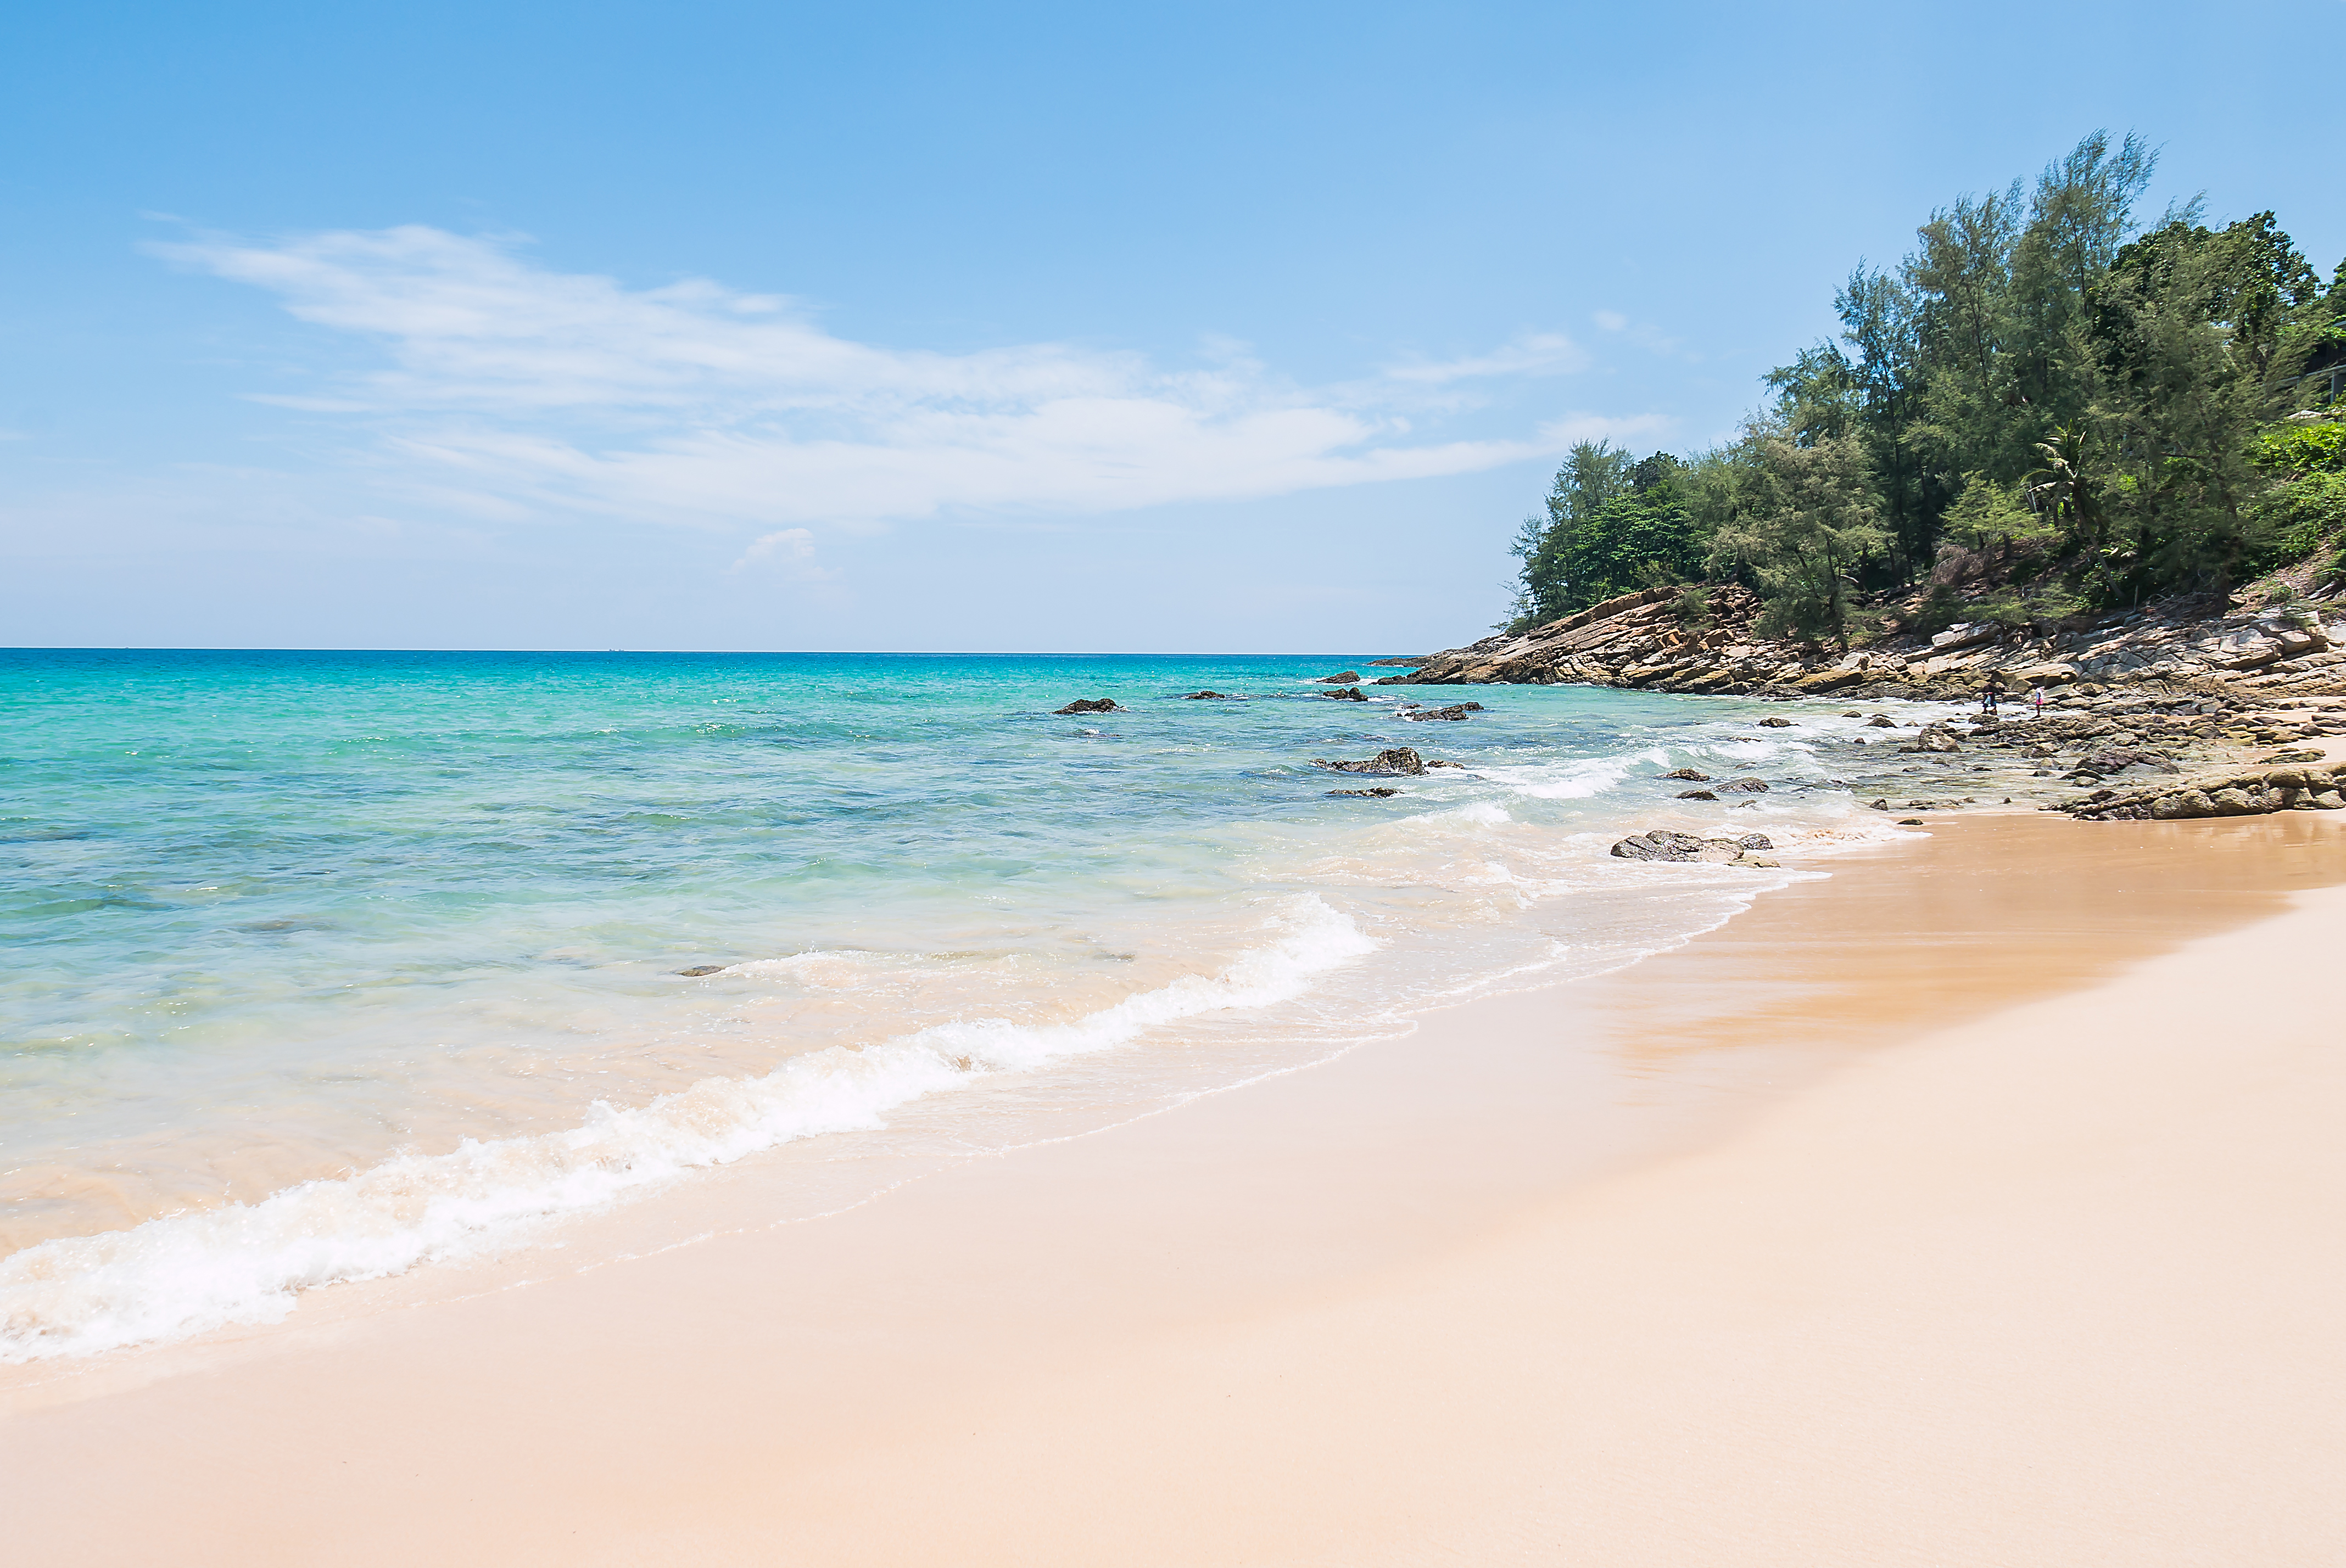
\includegraphics[width=\paperwidth]{tropical-beach}}

\graphicspath{{include/}}

% trick taken from https://topanswers.xyz/tex?q=1989
\tikzset{
    use page relative coordinates/.style={
        shift={(current page.south west)},
        x={(current page.south east)},
        y={(current page.north west)}
    },
}

\usepackage{fontspec}
\newfontfamily\palmtree{Quivira}
\newfontfamily\palmtreeb{Twemoji Mozilla}[Renderer=Harfbuzz]
\newfontfamily\drumfont[Scale=5]{Segoe UI Symbol}
\ExplSyntaxOn
\newcommand\calcmodpage[2]{\int_eval:n{\int_mod:nn{\value{page}+#2}{#1}+1}}
\newcommand\drumstickrotate{%
 \int_compare:nNnTF{\int_mod:nn{\value{page}}{16}}<{8}
  {\def\myrotate{-80}}
  {\def\myrotate{-100}}}
\ExplSyntaxOff
\tikzset{drumstick/.pic={\fill[rounded corners=1] (0,0) rectangle (0.1,0.9);\fill[rounded corners=1,gray!30!black](0,0) rectangle (0.1,0.2);}}

\begin{document}

\begin{frame}
  \begin{tikzpicture}[remember picture, overlay]
    \begin{scope}[use page relative coordinates]
    \node[anchor=south west,inner sep=0pt,font=\palmtree\fontsize{10cm}{10cm}\selectfont]
    at (0.3,0.3){\textcolor{PaleGreen4}{\symbol{"1F334}}};
      \node[anchor=south,inner sep=0pt,font=\palmtreeb\fontsize{7cm}{7cm}\selectfont,rotate=5]
    at (0.2,0.15){\textcolor{PaleGreen4!90!black}{\symbol{"1F334}}};
    \node[anchor=south,xscale=-1,inner sep=0pt,font=\palmtreeb\fontsize{7cm}{7cm}\selectfont,rotate=7]
    at (0.7,0.2){\textcolor{PaleGreen3!90!black}{\symbol{"1F334}}};
     \node[anchor=south,inner sep=0pt,font=\palmtree\fontsize{10cm}{10cm}\selectfont,rotate=8]
    at (0.4,0.1){\textcolor{PaleGreen3!95!black}{\symbol{"1F334}}};
    \node at (0.1,0.58) {\includegraphics[width=0.6cm,page=\calcmodpage{59}{10}]{./include/bauble_bear}};
    \node at (0.3,0.83) {\includegraphics[width=0.6cm,page=\calcmodpage{59}{20}]{./include/bauble_coati}};
    \node at (0.08,0.77) {\includegraphics[width=0.5cm,page=\calcmodpage{59}{30}]{./include/bauble_koala}};
    \node at (0.25,0.6) {\includegraphics[width=0.5cm,page=\calcmodpage{59}{0}]{./include/bauble_marmot}};
    \node at (0.4,0.59) {\includegraphics[width=0.5cm,page=\calcmodpage{59}{50}]{./include/bauble_owl}};
    \node at (0.5,0.65) {\includegraphics[width=0.5cm,page=\calcmodpage{59}{45}]{./include/bauble_pingue}};
    \node at (0.6,0.64) {\includegraphics[width=0.5cm,page=\calcmodpage{59}{45}]{./include/bauble_duck}};
    \node at (0.4,0.94) {\includegraphics[width=0.5cm,page=\calcmodpage{59}{45}]{./include/bauble_duck}};
    \node at (0.9,0.72) {\includegraphics[width=0.5cm,page=\calcmodpage{59}{10}]{./include/bauble_koala}};
    \node at (0.8,0.62) {\includegraphics[width=0.5cm,page=\calcmodpage{59}{30}]{./include/bauble_bear}};
    \end{scope}
    \path
      (0.5\textwidth,-0.4\textheight) pic[thing/santa=red!80!black]{coati}
      (0.65\textwidth,-0.4\textheight) pic[thing/santa=yellow]{coati}
      (0.8\textwidth,-0.4\textheight) pic[thing/santa=black]{coati}
      (0.95\textwidth,-0.4\textheight) pic[thing/santa=green!80!black]{coati};
   \path
      (0.5\textwidth,-0.4\textheight) node[font=\drumfont]{\symbol{"1F6E2}}
      (0.65\textwidth,-0.4\textheight) node[font=\drumfont,text=red!80!black]{\symbol{"1F6E2}}
      (0.8\textwidth,-0.4\textheight) node[font=\drumfont,text=yellow]{\symbol{"1F6E2}}
      (0.95\textwidth,-0.4\textheight) node[font=\drumfont,text=green!80!black]{\symbol{"1F6E2}};

    \drumstickrotate
    \path
      (0.44\textwidth,-0.31\textheight) pic[yellow,rotate=\myrotate]{drumstick}
      (0.59\textwidth,-0.31\textheight)pic[green!80!black,rotate=\myrotate]{drumstick}
      (0.74\textwidth,-0.31\textheight) pic[red!80!black,rotate=\myrotate]{drumstick}
      (0.89\textwidth,-0.31\textheight) pic[black,rotate=\myrotate]{drumstick};
    \node[black,text width=.7\paperwidth,font=\tiny,align=center] at ([yshift=0.35cm]current page.south) {Image source: \url{https://www.freepik.com/free-photo/tropical-beach_1035215.htm}};
  \end{tikzpicture}%
  \pause[540]
\end{frame}

\end{document}